\usetikzlibrary{arrows.meta}%
\definecolor{myblue}{HTML}{1E88E5}%
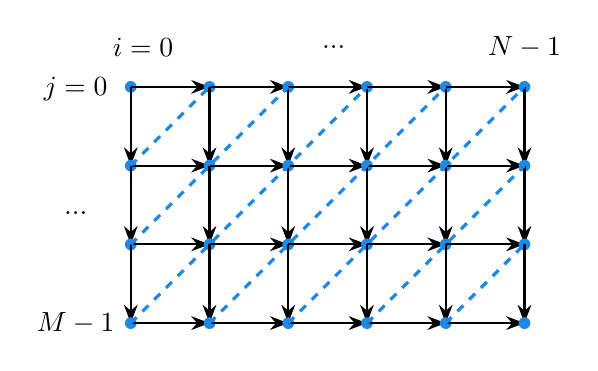
\begin{tikzpicture}[
    y=-1cm, % Flip the y-axis so (0,0) is at top left
    node/.style={circle, fill=myblue, inner sep=1.5pt},
    arr/.style={-{Stealth}, line width=0.8pt}
]
\def\N{5}
\def\M{3}
\foreach \i in {0,...,\N} {
    \foreach \j in {0,...,\M} {
        \node[node] at (\i,\j) {};
        \ifnum\i<\N
            \draw[arr] (\i,\j) -- (\i+1,\j);
        \fi
        \ifnum\j<\M
            \draw[arr] (\i,\j) -- (\i,\j+1);
        \fi
    }
}
\foreach \d in {0,...,\numexpr\N+\M\relax} {
    \pgfmathsetmacro{\startx}{max(0, \d-\M)}
    \pgfmathsetmacro{\starty}{min(\d, \M)}
    \pgfmathsetmacro{\endx}{min(\d, \N)}
    \pgfmathsetmacro{\endy}{max(0, \d-\N)}
    \pgfmathparse{(\startx != \endx) || (\starty != \endy) ? 1 : 0}
    \ifnum\pgfmathresult=1
        \draw[myblue, dashed, line width=1.2pt] (\startx,\starty) -- (\endx,\endy);
    \fi
}
\draw[draw=none] (\N,-0.5) -| (-0.7,\M)
  node[pos=0]{$N-1$}
  node[pos=0.2125]{...}
  node[pos=0.425]{$i=0$}
  node[pos=0.575]{$j=0$}
  node[pos=0.8]{...}
  node[pos=1]{$M-1$};
\end{tikzpicture}

